\section{Creazione del training set}
Il dataset in input è stato prodotto a seguito delle operazioni di data integration su tre dataset originari. Durante queste operazioni, gli attributi privi di informazioi rilevanti ai fini dell'addestramento di un modello di Machine Learning sono stati rimossi, ottenendo un dataset già pronto all'uso. Per dividere il dataset in train set e test set, è stata definita una funzione ad hoc che permette di dividere il dataset in 10 parti, usandone poi 9 per il trainset e la restante per il testset. Questa funzione si è rivelata fondamentale per l'operazione di 10-fold cross validation, in cui il modello viene addestrato e testato su porzioni differenti del dataset.

\section{Analisi esplorativa del dataset}
\todo{Controllare eventiali affermazioni "forti" MM}
\todo{Posizionamneto figure MM}
Ai fini di evidenziare la distribuzione dei dati rispetto ai vari attributi del dataset, è stata condotta un'analisi esplorativa del dataset mediante funzioni statistiche del linguaggio R.\\
I dataset è formato da 312895 sample, 7 feature e una etichetta a 2 livelli.
Tramite la funzione \texttt{sapply(dataset, class)} è stata ottenuta la classe di ogni feature, che è stata poi sottoposta ad un'analisi più approfondita.\\
L'attributo Country è un attributo stringa fattorizzato, che presenta 21 livelli. Il valore più frequentemente riportato è "United States", seguito da "United Kindom" e "Canada".\\
L'attributo GDP per capita è un attributo numerico di valore intero continuo che rappresenta il guadagno annuo medio nello stato in cui il progetto è stato proposto. La distribuzione dei due attributi sopracitati è mostrata in Figura \ref{fig:countrygdp}. Notiamo che per entrambi i grafici è stata utilizzata la scala logaritmica, in quanto la frequenza associata ad alcuni valori è molto alta. In particolare abbiamo notato che la maggior parte dei progetti (oltre il 70\%) è stato creato negli Stati Uniti.

\begin{figure}%
	\centering
	\subfloat[Distribuzione dell'attributo Country. Si noti che l'asse y è riportato in scala logaritmica.]{{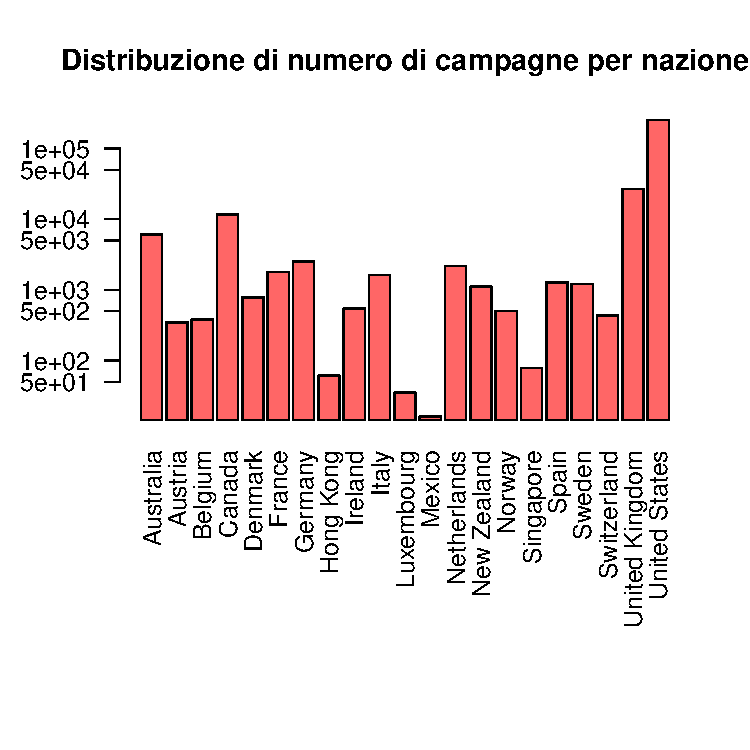
\includegraphics[width=0.45\linewidth]{../FinalResults/Images/Data_exploration_plots/barlpot_country} }}%
	\qquad
	\subfloat[Distribuzione dell'attributo rappresentante il GDP pro capite]{{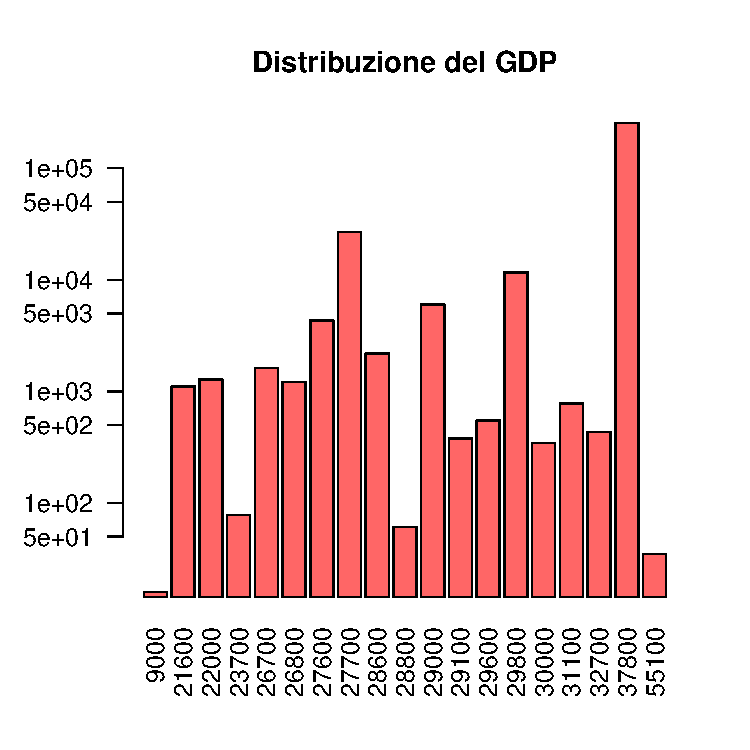
\includegraphics[width=0.45\linewidth]{../FinalResults/Images/Data_exploration_plots/barlpot_gdp}}}%
	\caption{}%
	\label{fig:countrygdp}%
\end{figure}

Sono poi stati analizzati gli attributi relativi alle categorie dei progetti proposti, quindi le feature main category e category. Entrambi i campi, costituiti da stringhe fattorizzate, si mostrano distribuite in modo sostanzialmente uguale tra i possibili valori, come mostrato nella Figura \ref{fig:piecategory}. 

\begin{figure}%
	\centering
	\subfloat[Distribuzione dell'attributo rappresentante la categoria specifica del progetto.]{{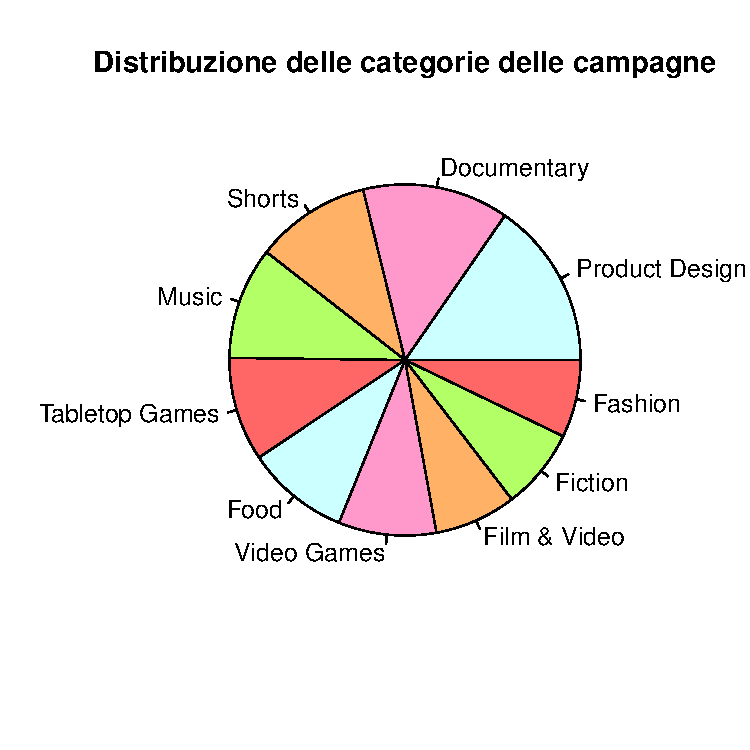
\includegraphics[width=0.45\linewidth]{../FinalResults/Images/Data_exploration_plots/pie_categories} }}%
	\qquad
	\subfloat[Distribuzione dell'attributo rappresentante la categoria generale del progetto.]{{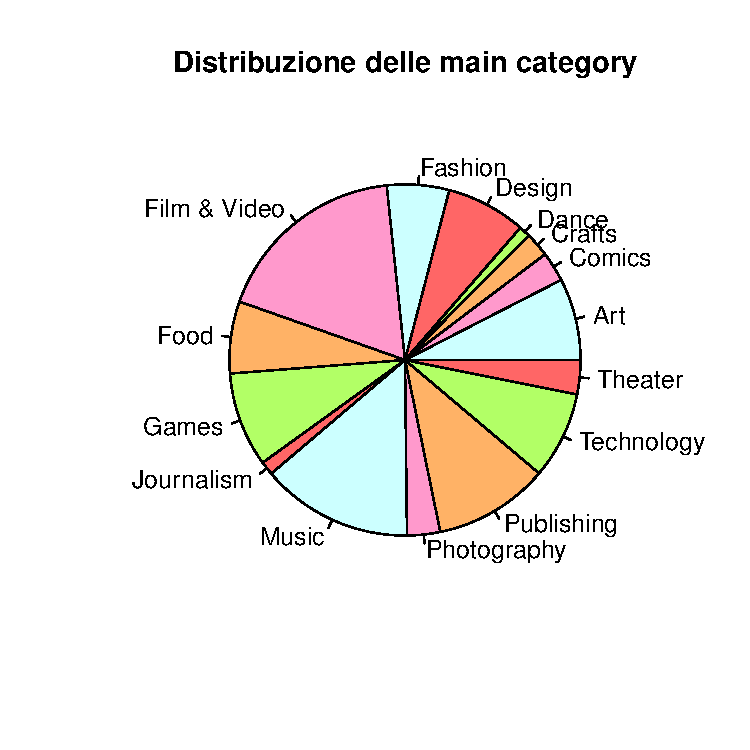
\includegraphics[width=0.45\linewidth]{../FinalResults/Images/Data_exploration_plots/pie_main_category}}}%
	\caption{}%
	\label{fig:piecategory}%
\end{figure}

La distribuzione del campo service (Figura \ref{fig:barlpotservice}), rappresentante la percentuale di sviluppo dei settori terziari nel paese in cui è stato proposto il progetto, mostra come la maggior parte dei sample sia relativa a paesi con un settore terziario predominante sugli altri due.   

\begin{figure}
	\centering
	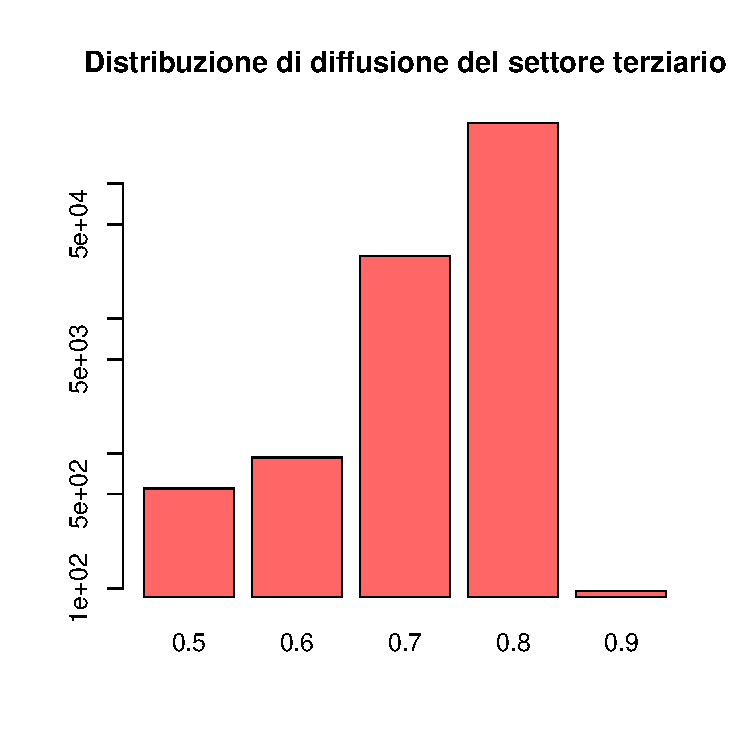
\includegraphics[width=0.7\linewidth]{../FinalResults/Images/Data_exploration_plots/barlpot_service}
	\caption{Distribuzione dell'attributo service.}
	\label{fig:barlpotservice}
\end{figure}

Le feature goal e backer sono due attributi interi e continui che rappresentano rispettivamente la richiesta minima di denaro al fine di considerare il progetto riuscito ed il numero di donatori. Per questi due campi sono stati analizzati il valore medio e la deviazione standard; i risultati ottenuti sono stati riportati nella Tabella \ref{tab:meansdgoalbackers}. Un valore così elevato di deviazione standard rispetto alla media, indica che i dati sono caratterizzata da una significativa varietà e distanza dal valore medio riportato.
\begin{table}
	\centering
	\label{tab:meansdgoalbackers}
	\caption{Media e deviazione standard degli attributi goal e backers}
	\begin{tabular}{|c|c|c|}
		\hline 
		\textbf{Feature} & \textbf{Valore medio} & \textbf{Deviazione standard} \\ 
		\hline 
		goal & 46672.68 & 1112774 \\ 
		\hline 
		backers & 102.98 & 946.76 \\ 
		\hline 
	\end{tabular} 
\end{table}


L'ultimo aspetto analizzato è stata la distribuzione dell'etichettatura dei progetti, per capire come fossero divise le tuple all'interno del nostro dataset. Come mostrato in Figura , la maggioranza dei sample (63\%) in nostro possesso risultano essere relativi a progetti fallimentari. Il numero non risulta comunque tanto squilibrato da generare problemi nella fase di addestramento dei modelli di Machine Learning.

\begin{figure}
	\centering
	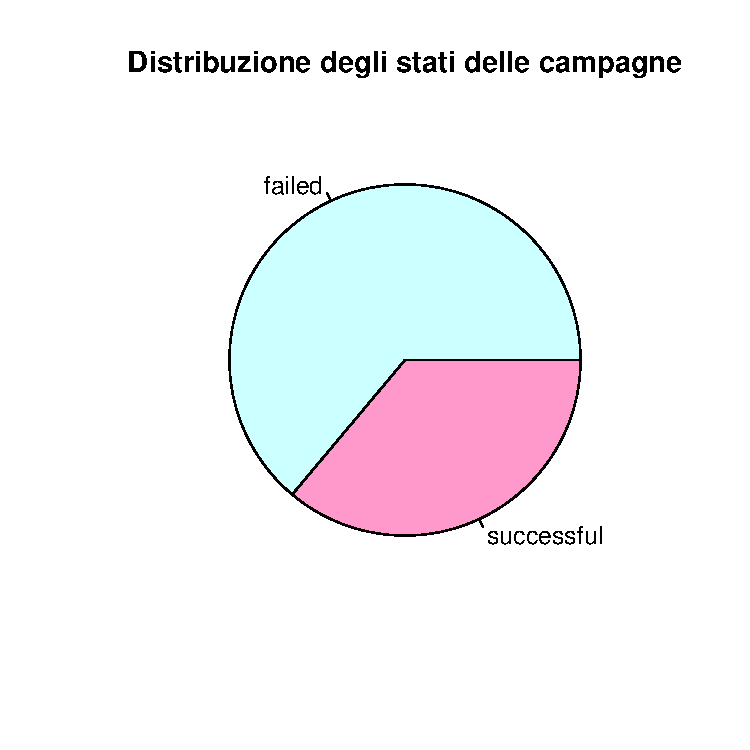
\includegraphics[width=0.8\linewidth]{../FinalResults/Images/Data_exploration_plots/pie_state}
	\caption{Distribuzione dell'attributo state, l'etichetta dei nostri sample.}
	\label{fig:piestate}
\end{figure}


È stata infine prodotta la matrice di correlazione (mostrata in Figura \ref{fig:corrplot}) tra i vari attributi del dataset; come previsto, è emersa una evidente correlazione tra il paese in cui il progetto viene creato e i campi relativi al GDP pro capite e alla percentuale di diffusione del settore terziario nello stato. Questo poichè questi valori provengono da un dataset esterno joinato al dataset dei progetti Kickstarter proprio sul campo nazione. Dalla matrice non emergono altre correlazioni rilevanti tra i restanti attributi del dataset.

\begin{figure}
	\centering
	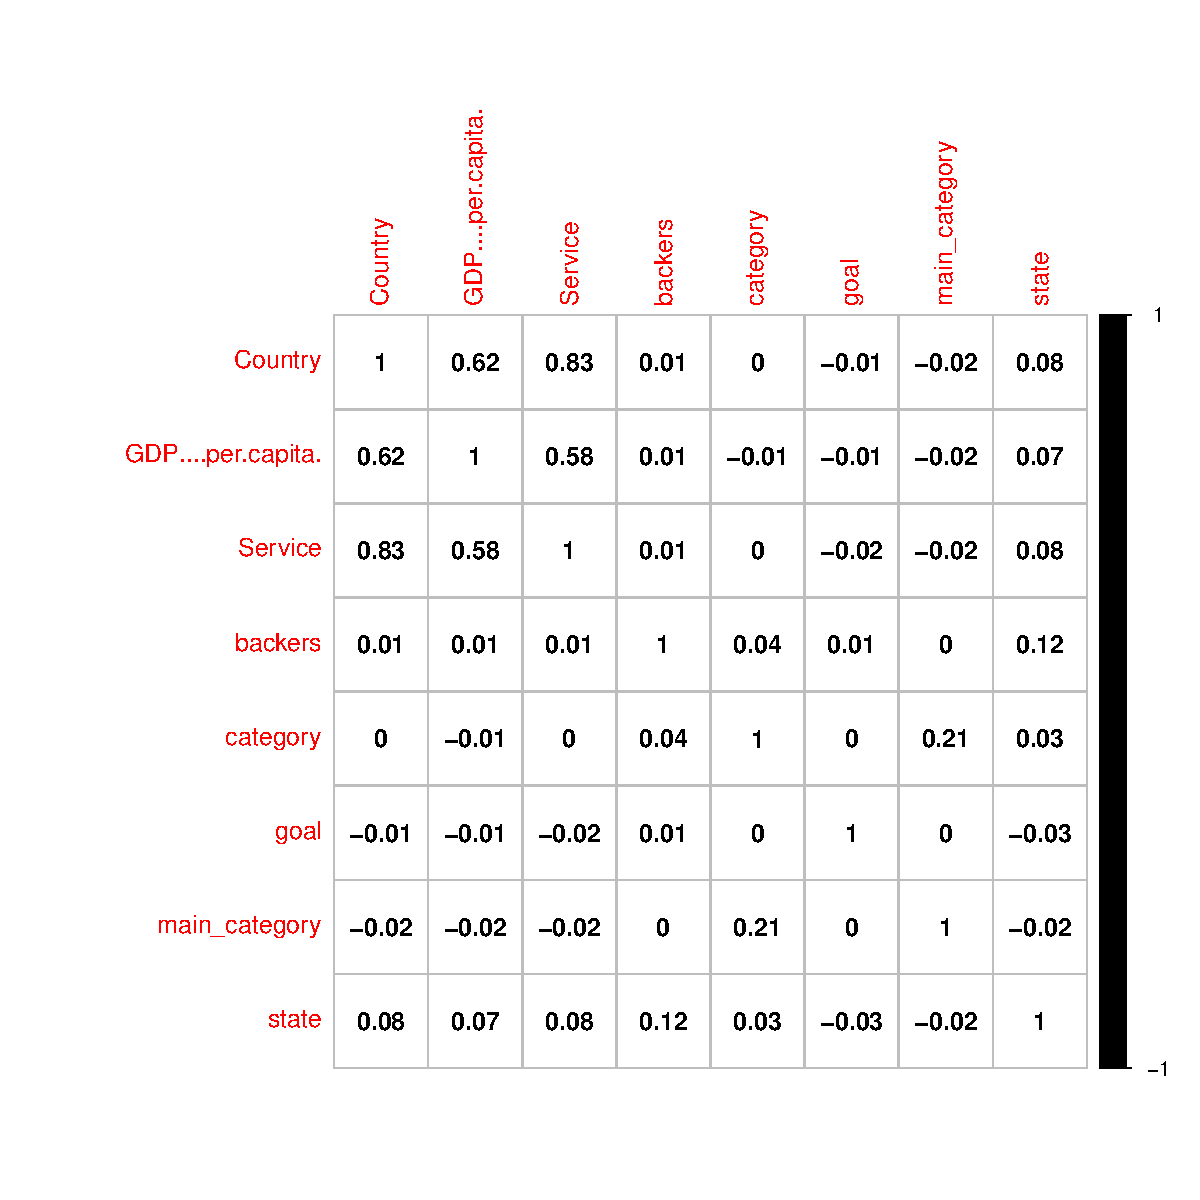
\includegraphics[width=1\linewidth]{../FinalResults/Images/Data_exploration_plots/corrplot}
	\caption{Matrice di correlazione tra le feature del dataset.}
	\label{fig:corrplot}
\end{figure}


\section{Modelli di Machine Learning utilizzati}
Al fine di avere una misura di riferimento per i modelli che saranno proposti successivamente, è stato prodotto un modello baseline, che si limita a rispondere sempre failed ad ogni sottomissione di un sample. La risposta risulta essere sempre failed in quanto, dall'analisi esplorativa dei dati effettuata in precedente, è emerso che il valore di etichettatura più frequente era prorpio il fallimento del progetto.\\
In Figura \ref{fig:baselineperformance} sono riporatte le misure di performance ottenute con questo modello a seguito dell'operazione di 10 fold cross validation; notiamo come accuratezza e precisione si uniformino alla distribuzione delle etichettature failed nel dataset, mentre la recall rimanga ovviamente fissa ad 1.\\
Le curve ROC associate a questo modello, ripotate in Figura \ref{fig:baselineROC}, restituiscono un valore della Area Under Curve (AUC) molto variabile: ciò è dovuto dalla diversa distribuzione dei sample con etichettatura failed all'interno dei testset prodotti dal porcesso di 10-fold cross validation.

\begin{figure}
	\centering
	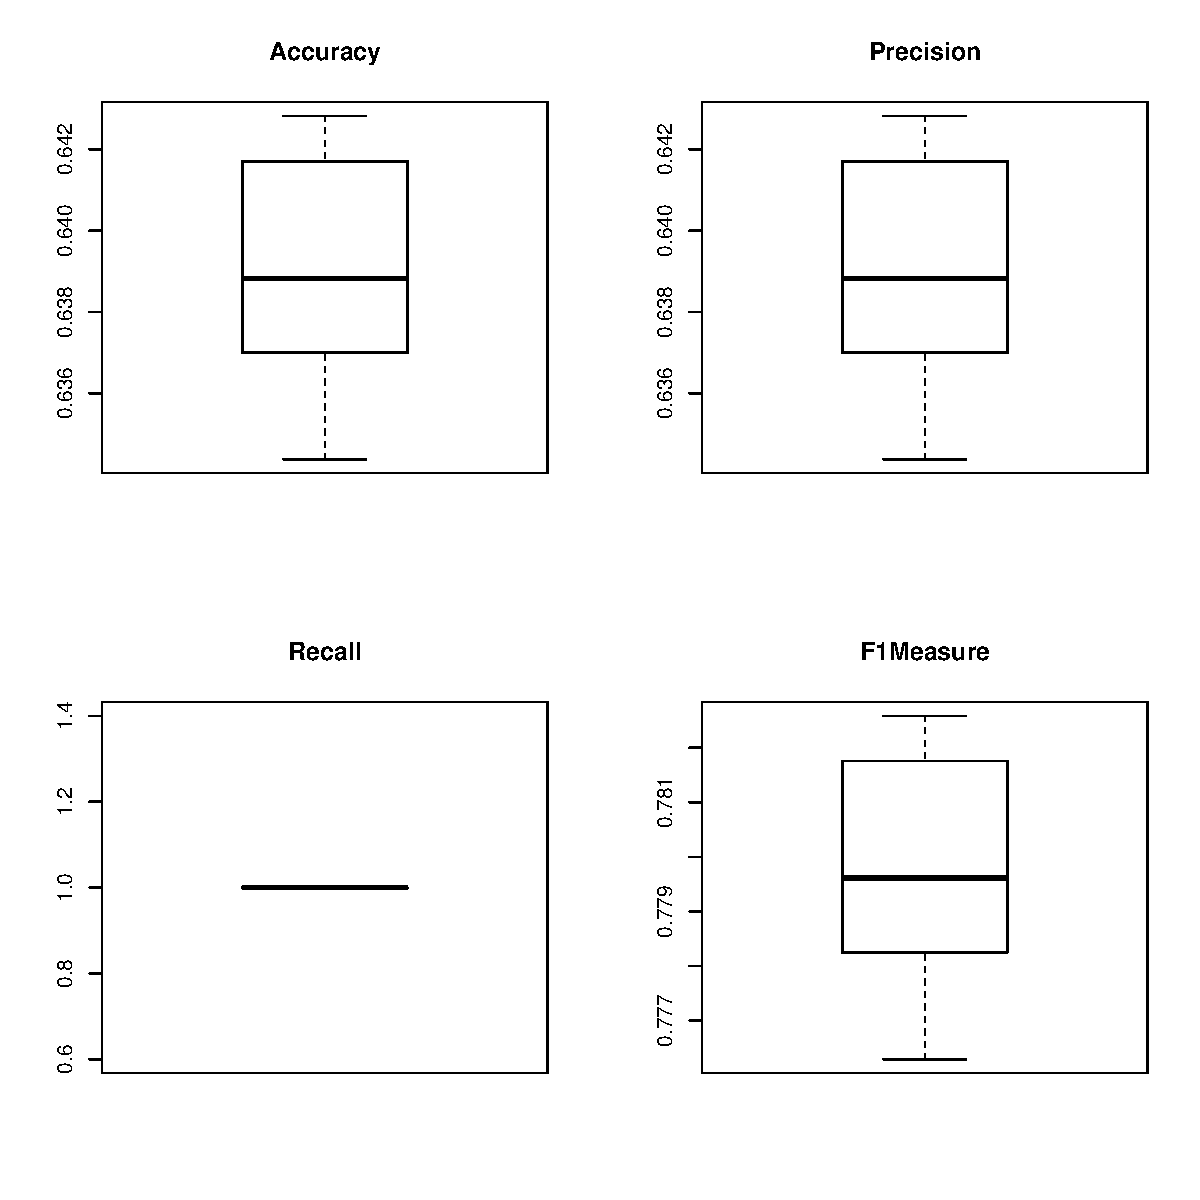
\includegraphics[width=0.7\linewidth]{../FinalResults/Baseline_performance}
	\caption{Boxplot relativi alle misure di performance del modello baseline.}
	\label{fig:baselineperformance}
\end{figure}

\begin{figure}
	\centering
	\subfloat{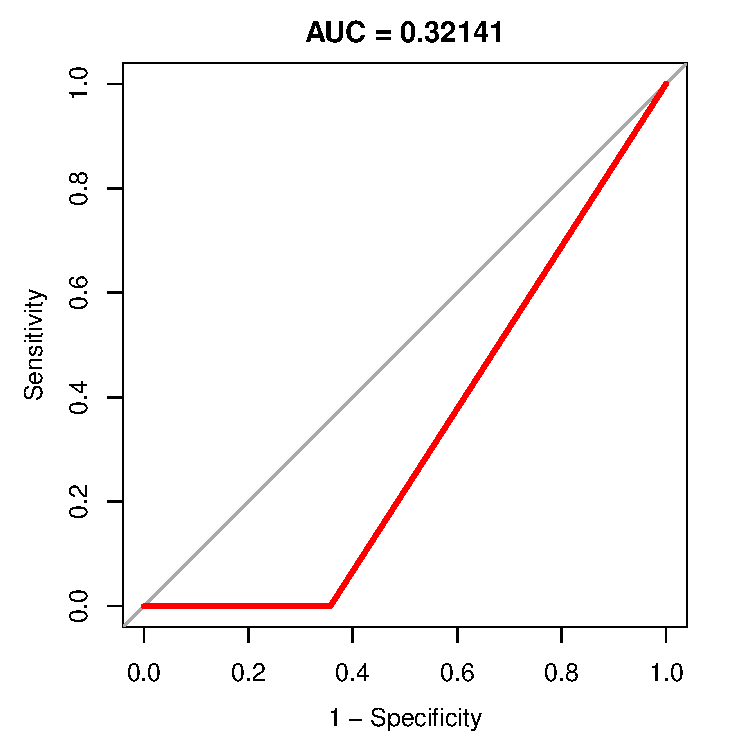
\includegraphics[width=0.3\linewidth]{../FinalResults/Images/baseline/auc_1.pdf}}\quad
	\subfloat{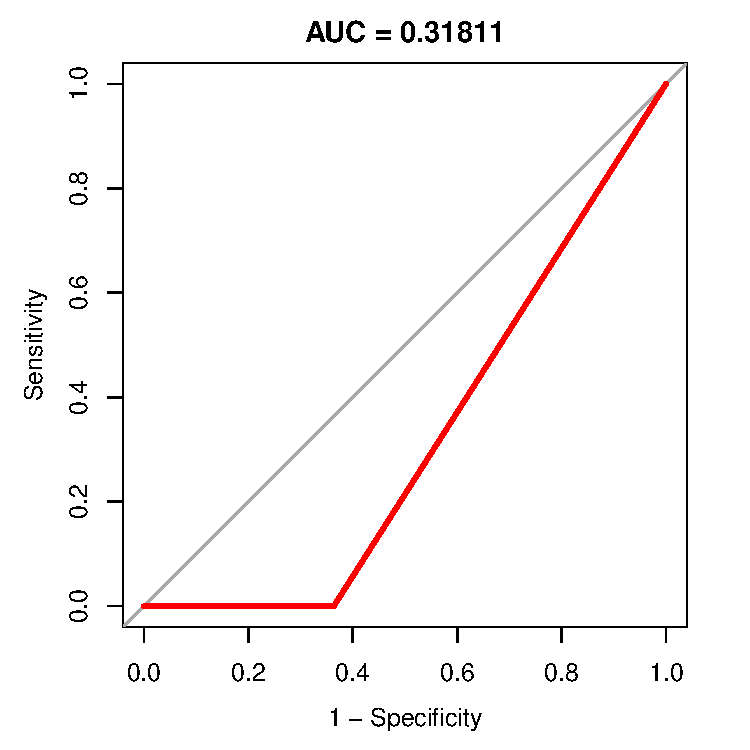
\includegraphics[width=0.3\linewidth]{../FinalResults/Images/baseline/auc_2.pdf}}\quad
	\subfloat{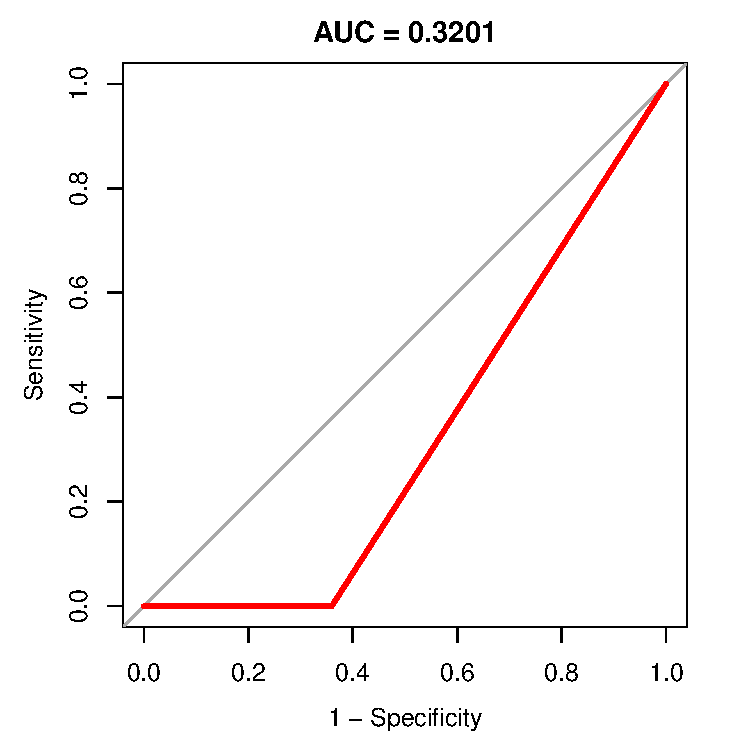
\includegraphics[width=0.3\linewidth]{../FinalResults/Images/baseline/auc_3.pdf}}\quad
	\subfloat{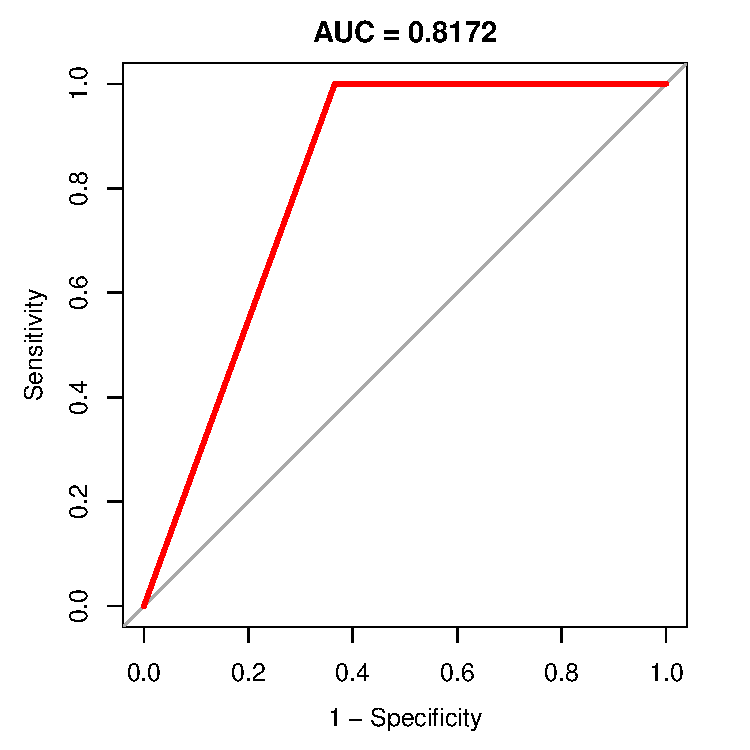
\includegraphics[width=0.3\linewidth]{../FinalResults/Images/baseline/auc_4.pdf}}\quad
	\subfloat{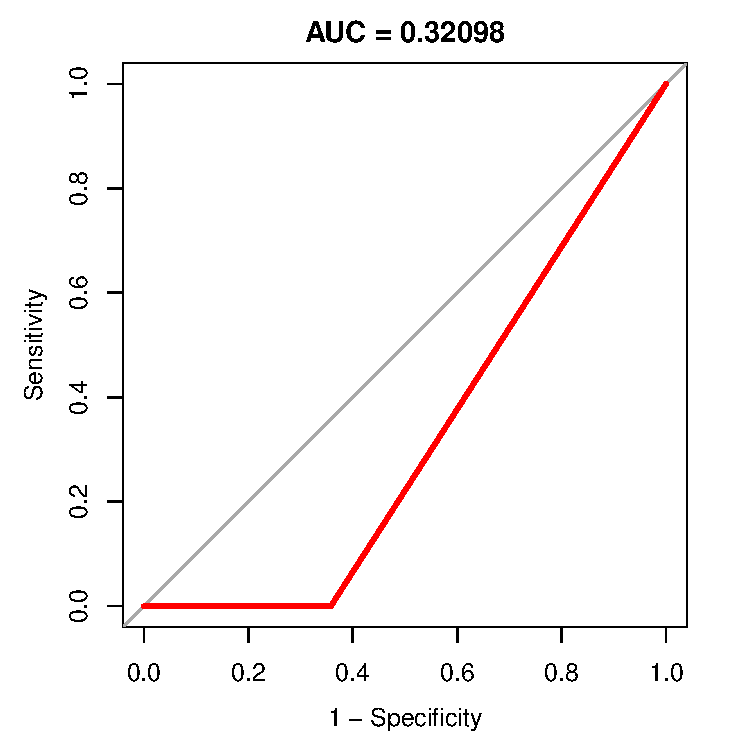
\includegraphics[width=0.3\linewidth]{../FinalResults/Images/baseline/auc_5.pdf}}\quad
	\subfloat{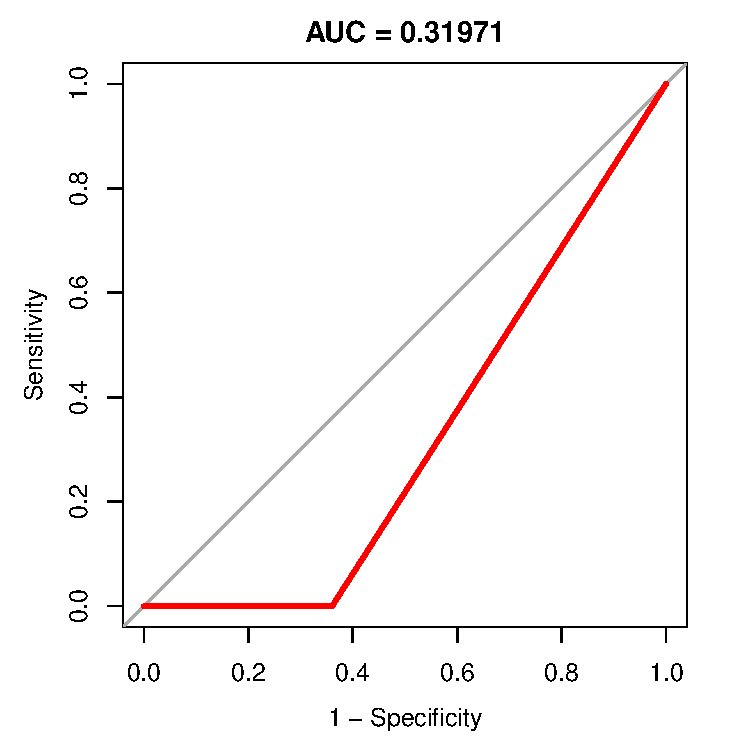
\includegraphics[width=0.3\linewidth]{../FinalResults/Images/baseline/auc_6.pdf}}\quad
	\subfloat{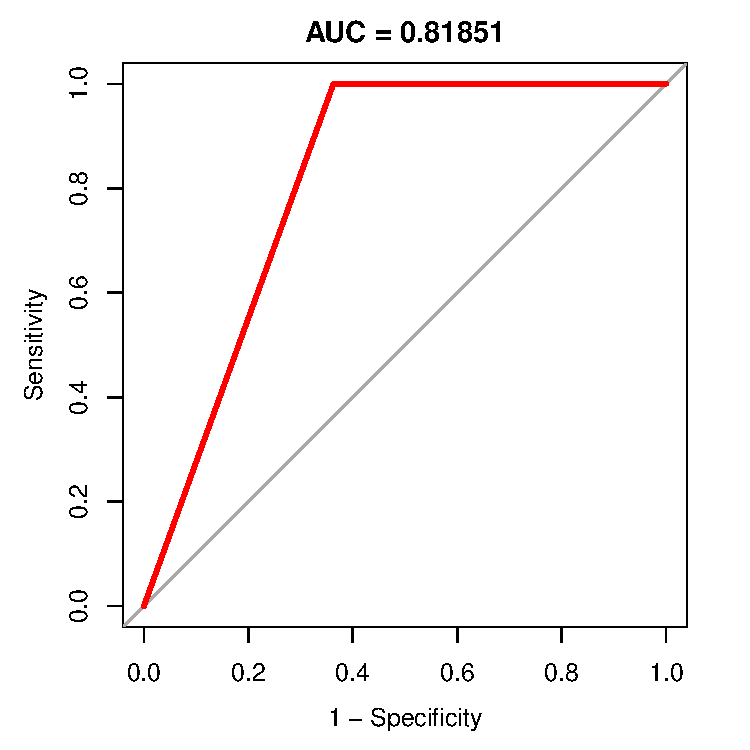
\includegraphics[width=0.3\linewidth]{../FinalResults/Images/baseline/auc_7.pdf}}\quad
	\subfloat{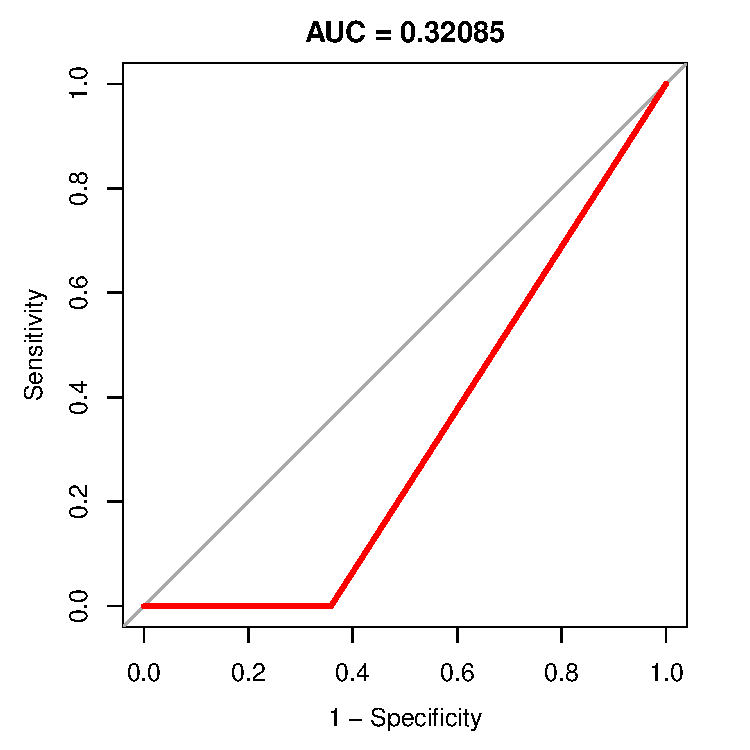
\includegraphics[width=0.3\linewidth]{../FinalResults/Images/baseline/auc_8.pdf}}\quad
	\subfloat{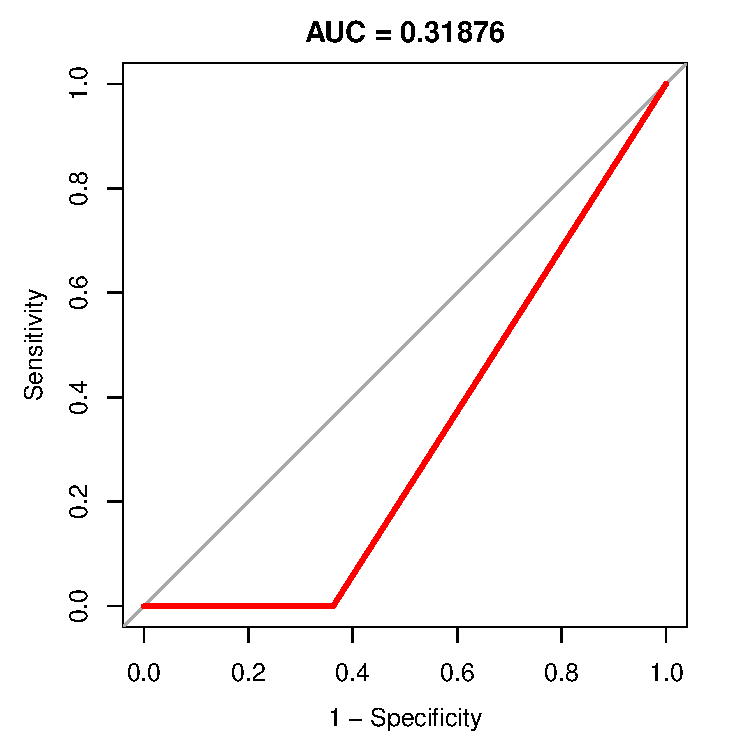
\includegraphics[width=0.3\linewidth]{../FinalResults/Images/baseline/auc_9.pdf}}\quad
	\subfloat{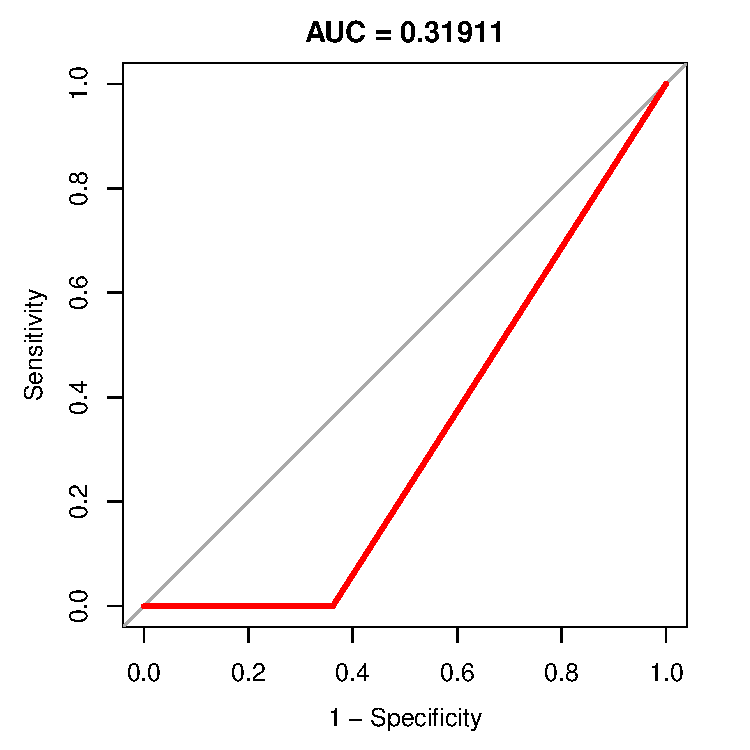
\includegraphics[width=0.3\linewidth]{../FinalResults/Images/baseline/auc_10.pdf}}\quad
	\caption{Curve ROC del modello baseline per la 10-fold cross validation.}
	\label{fig:baselineROC}
\end{figure}       

\subsection{Alberi decisionali}
\subsection{Reti neurali}
\subsection{Support Vector Machine}
\subsection{Naive Baies}